\documentclass[a4paper, 12pt, conference]{ieeeconf} 
\overrideIEEEmargins
\usepackage[italian]{babel} % imposta lingua
\usepackage[utf8]{inputenc} % imposta lingua
\usepackage[babel]{csquotes} % imposta lingua
\usepackage[T1]{fontenc} % imposta lingua
\usepackage{amsmath, amssymb, amsfonts} % pachetto per formule
% \usepackage[parfill]{parskip} % non si dovrebbe fare, ma sostituisce le rientranze dei paragrafi con interlinea
\usepackage{listings} % per poter far riconoscere e colorare codice 
\usepackage{xcolor} % pacchetto per testo colorato
\usepackage{float, subfig} % pachetto per figure, per posizionamento
\usepackage{booktabs} % pacchetto per tabelle
\usepackage{graphicx, wrapfig} % pachetto per tabelle
\usepackage{tcolorbox} % riquadri colorati
\usepackage[Listato]{algorithm} % pseudocodice
\usepackage{algpseudocode} % pseudocodice
\usepackage[hidelinks]{hyperref} % indice e riferimenti cliccabili e senza riquadro rosso
\frenchspacing %spaziatura italiana per accenti
\usepackage[colorinlistoftodos,prependcaption,textsize=tiny]{todonotes} % note TODO
% CONFIGURAZIONE LINK E RIFERIMENTI
\hypersetup{%
	pdfpagemode={UseOutlines},
	bookmarksopen,
	pdfstartview={FitH},
	colorlinks,
	linkcolor={black}, %COLORE DEI RIFERIMENTI AL TESTO
	citecolor={blue}, %COLORE DEI RIFERIMENTI ALLE CITAZIONI
	urlcolor={blue} %COLORI DEGLI URL
}

\title{\LARGE \bf
Performance Time Report
}

\author{Mistri Matteo - 808097\\
	Daniele Maria Papetti - 808027
}


\begin{document}


\twocolumn[
\begin{@twocolumnfalse} 
\maketitle
\thispagestyle{empty}
\pagestyle{empty}
\rule{\textwidth}{.5pt}
\begin{abstract}

Il cancro alla cervice uterina è una delle forme di tumore più diffuse tra le donne, con un tasso di mortalità superiore al $50\%$.
Nonostante sia possibile individuarlo durante le fasi iniziali del suo sviluppo grazie a un continuo monitoraggio, in aree del mondo meno sviluppate ciò non è sempre possibile, portando così ad un incremento del tasso di mortalità.
%In questo lavoro si cerca di sviluppare un modello che ha lo scopo di aiutare i medici nel processo di diagnosi di tale patologia. 
L'obiettivo principale di questo lavoro è quello di produrre un modello di \textit{machine learning} in grado di predire se un soggetto, in funzione di un insieme di caratteristiche, sia affetto o meno dalla patologia.
Il dataset utilizzato contiene le informazioni di $858$ pazienti, i cui dati sono stati raccolti in un ospedale di Caracas \cite{ML}.
Studi esplorativi del dataset evidenziano come il problema sia estremamente sbilanciato (10 - 90) in favore della classe rappresentante l'assenza del tumore.
%Studi esplorativi del dataset evidenziano come il problema trattato sia binario (\textit{i.e.}, il paziente soffre o no della patologia) ed estremamente sbilanciato (10 - 90) in favore della classe rappresentante l'assenza del tumore.
Dopo aver effettuato alcune operazioni di \textit{preprocessing} sui dati, si è deciso di addestrare due differenti modelli per ognuno dei tre input generati (decision tree e random forest).
%I modelli indagati sono stati i DT (decision tree) e le RF (random forest), in quanto risultano essere entrambi modelli \textit{explainable}; questa caratteristica risulta essere molto apprezzata in ambito medico, in quanto si è in grado di motivare le risposte fornite dal modello di apprendimento automatico.
I possibili input utilizzati per ogni modello sono il dataset senza nessun operazione di feature reduction, il dataset dopo l'operazione di feature selection basata su correlazione e infine le feature estratte mediante il processo della Principal Component Analysis (PCA).
%Poiché sia la PCA che la feature selection sfruttano un iperparametro (\textit{e.g.}, il numero di componenti prodotti dalla PCA), sono stati effettuati degli studi preliminari su questi iperparametri in modo da selezionare dei relativi valori ottimali.
I vari modelli prodotti sono stati valutati secondo un procedimento di 5-fold \textit{stratified cross-validation}, utilizzando come metrica utilizzata la f1-\textit{measure} rispetto alla classe minoritaria (\textit{i.e.}, biopsia positiva).
%Per favorire l'apprendimento del modello, i train set, ad ogni iterazione del processo, sono stati arricchiti mediante la tecnica di \textit{oversampling} SMOTE (Synthetic Minority Over-sampling TEchnique).
Il confronto tra i modelli è stato effettuato sfruttando dei \textit{paired} t-test, prima tra i due modelli appartenenti al medesimo input e poi tra i migliori di ogni strategia.
I risultati evidenziano l'assenza di differenze statistiche tra i modelli addestrati sfruttando l'intero dataset o con le feature prodotte dal processo di PCA, mentre le Random Forest (RF) risultano statisticamente migliori del Decision Tree (DT) nel caso dell'operazione di feature selection mediante correlazione; i confronti tra i modelli con input differenti non hanno evidenziato differenze statisticamente rilevanti.
%I confronti tra le RF ottenute dai vari metodi evidenziano che non è possibile stabilire differenze statisticamente significative tra esse.
Infine, gli algoritmi di apprendimento automatico utilizzati in precedenza sono stati addestrati sfruttando il dataset privato delle feature riguardanti gli esiti dei test clinici.
I risultati evidenziano che l'assenza di queste informazioni pregiudica fortemente la discriminazione della classe positiva da quella negativa, confermando l'importanza di tali esami.
\end{abstract}
\rule{\textwidth}{.5pt}
\end{@twocolumnfalse}
]

\section{INTRODUCTION}
Il cancro alla cervice uterina è la terza forma di tumore più diffusa tra le donne, dopo quelle al seno e al colon-retto. La patologia aggredisce le cellule del collo dell’utero, ovvero il segmento che pone in collegamento l’utero con la vagina. Rispetto ad altre neoplasie, il tumore della cervice uterina ha il vantaggio di essere del tutto prevenibile e comunque ben curabile se rilevato precocemente \cite{veronesi}.
Nonostante la possibilità di prevenzione offerta da uno screening citologico regolare, questa forma di tumore colpisce oltre mezzo milione di donne all'anno, con un tasso di mortalità di oltre il $50\%$; la maggioranza dei decessi avviene in aree del mondo poco sviluppato, dove non è disponibile un meccanismo di screening regolare e sistematico sulla popolazione, che permetterebbe un riconoscimento precoce delle lesioni che precedono il tumore, permettendo così un intervento tempestivo dei medici \cite{paper}.
I maggiori fattori di rischio, che favoriscono la comparsa di questo tipo di cancro, sono individuabili principalmente nelle malattie sessualmente trasmissibili, in particolare nel Papilloma virus.\\
In questo lavoro, è stato utilizzato un dataset contenete i dettagli di anamnesi ed esami clinici relativi a un campione di $858$ donne al fine di stabilire se sia possibile realizzare un modello di predizione efficace per stabilire l'esito della biopsia del tessuto uterino a partire dai dati raccolti.
In particolare, sono stati messi a confronto diversi modelli di apprendimento automatico considerati \textit{explainable}, ovvero in grado di motivare il risultato della predizione fornita, in quanto in ambito medico modelli \textit{black box} risultano spesso non adatti per via della bassa interpretabilità da parte dei medici.
Gli obiettivi di questo lavoro possono essere riassunti come segue:
\begin{itemize}
	\item esplorazione e pulizia del dataset;
	\item confronto di differenti tecniche di feature reduction;
	\item addestramento di vari modelli per predire si i soggetti sono affetti dalla patologia;
	\item confronto dei vari modelli al fine di determinare quello con performance ottimali.
\end{itemize}
Il report è stato suddiviso nelle seguenti sezioni: (II) introduzione al dataset e operazioni di esplorazione e pulizia dei dati; (III) presentazioni dei metodi utilizzati per la creazione di una serie di modelli predittivi; (IV) presentazione ed analisi dei risultati ottenuti; (V) conclusioni e possibili sviluppi futuri.

\section{DATASET}
\subsection{Data exploration}
Il dataset fornito presenta $858$ sample, ognuno associato ad un totale di $36$ feature, etichetta inclusa. Un elenco di queste ultime è riportata in Tabella \ref{tab:attributes}, dove viene altresì riportato il DataType associato ad ognuno di essi. I dati provengono da uno screening effettuato su una popolazione di donne in un ospedale di Caracas, Venezuela \cite{ML}, delle quali sono stati raccolti e riportati una serie di dati personali, medici e strumentali. In particolare, nel dataset è possibile individuare un gruppo di feature relative all'attività sessuale delle donne, al numero di partner ed al tipo di contraccettivo utilizzato (ormonale vs intrauterino -IUD-). Viene poi riportata una lunga lista di malattie sessualmente trasmissibili (STDs), il numero totale di patologie sessuali contratte e l'intervallo di tempo trascorso dalla prima e dall'ultima diagnosi di queste malattie. Sono infine presenti informazioni circa precedenti diagnosi di cancro o Papilloma Virus (DX) e i risultati di alcuni esami strumentali eseguiti sulle pazienti. L'etichetta, ovvero la feature che deve venir predetto dal modello, è l'esito della Biopsia, un esame eseguito su una porzione del tessuto sospetto per accertare la presenza o meno di cellule tumorali attive. 
\begin{table}
	\centering
	\caption{Tabella riportante le feature presenti nel dataset ed il relativo tipo.}
	\label{tab:attributes}
	\begin{tabular}{|c|c|}
		\toprule 
		Feature & DataType \\ 
		\midrule 
		Age & Interval (Int) \\ 
		Number of sexual partners & Interval (Int) \\ 
		First sexual intercourse & Interval (Int) \\ 
		Num of pregnancies & Interval (Int) \\
		Smokes & Nominal (Bool) \\
		Smokes (years) & Ratio (Double) \\ 
		Smokes (packs/year) & Ratio (Double) \\ 
		Hormonal Contraceptives & Nominal (Bool) \\ 
		Hormonal Contraceptives (years) & Ratio (Double) \\ 
		IUD & Nominal (Bool) \\ 
		IUD (years) & Ratio (Double) \\ 
		STDs & Nominal (Bool) \\ 
		STDs (number) & Interval (Int) \\ 
		STDs:condylomatosis & Nominal (Bool) \\ 
		STDs:cervical condylomatosis & Nominal (Bool) \\ 
		STDs:vaginal condylomatosis & Nominal (Bool) \\ 
		STDs:vulvo-perineal condylomatosis & Nominal (Bool) \\ 
		STDs:syphilis & Nominal (Bool) \\ 
		STDs:pelvic inflammatory disease & Nominal (Bool) \\ 
		STDs:genital herpes & Nominal (Bool) \\ 
		STDs:molluscum contagiosum & Nominal (Bool) \\ 
		STDs:AIDS & Nominal (Bool) \\ 
		STDs:HIV & Nominal (Bool) \\ 
		STDs:Hepatitis B & Nominal (Bool) \\ 
		STDs:HPV & Nominal (Bool) \\ 
		STDs: Number of diagnosis & Interval (Int) \\
		STDs: Time since first diagnosis & Interval (Int) \\ 
		STDs: Time since last diagnosis & Interval (Int) \\ 
		Dx:Cancer & Nominal (Bool) \\ 
		Dx:CIN & Nominal (Bool) \\ 
		Dx:HPV & Nominal (Bool) \\ 
		Dx & Nominal (Bool) \\ 
		Hinselmann & Nominal (Bool) \\ 
		Schiller & Nominal (Bool) \\
		Citology & Nominal (Bool) \\ 
		Biopsy & Nominal (Bool) \\ 
		\bottomrule 
	\end{tabular} 
\end{table}

Lo studio della distribuzione dei valori (presenza o assenza di cellule tumorali) assunti dall'etichetta ha riportato un forte sbilanciamento delle classi, come rappresentato in Figura \ref{fig:biopsydistribution}, con solo $55$ sample ($6,4\%$ del totale) appartenenti alla classe positiva.
\begin{figure}
	\centering
	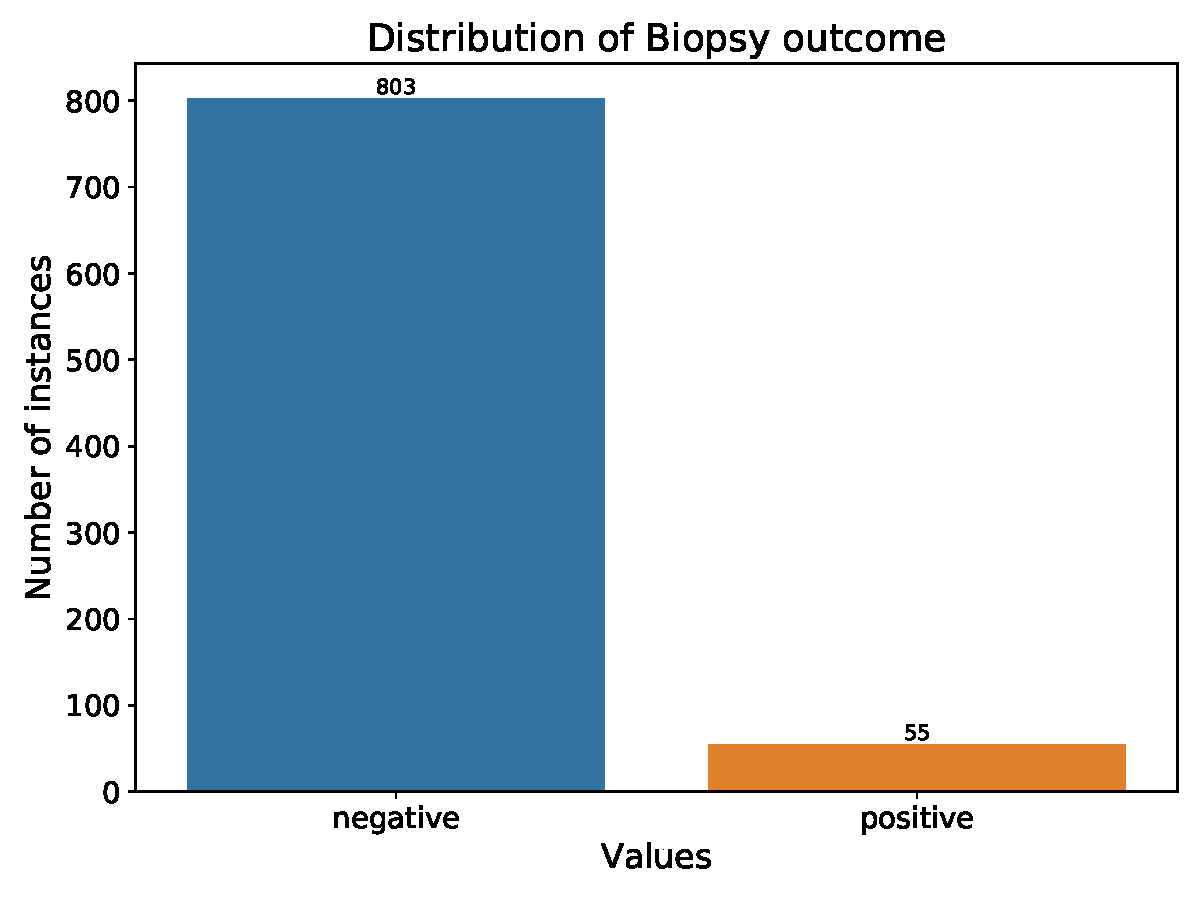
\includegraphics[width=1\linewidth]{images/biopsy_distribution}
	\caption{Distribuzione delle etichette all'interno del dataset. Il problema risulta fortemente sbilanciato verso la classe negativa.}
	\label{fig:biopsydistribution}
\end{figure}
A seguito della fase di \textit{Data cleaning}, presentata nella sottosezione successiva, è stato eseguito uno studio della correlazione tra le varie feature del dataset (inclusa l'etichetta). La Figura \ref{fig:corrmatrix} riporta la \textit{heatmap} associata ai valori di correlazione; da essa si evince la presenza di una forte correlazione interna tra le feature relative alle malattie sessualmente trasmissibili e tra gli esami di laboratorio e l'etichetta. Più in generale, è presente una correlazione elevata tra quelle coppie di feature che rappresentano il medesimo dato, in un caso tramite valore booleano, nell'altro mediante un dato numerico. Questa costatazione risulta in linea con le aspettative e suggerisce una presenza di ridondanza dell'informazione, risolvibile mediante l'utilizzo di tecniche di riduzione della dimensionalità.
\begin{figure}
	\centering
	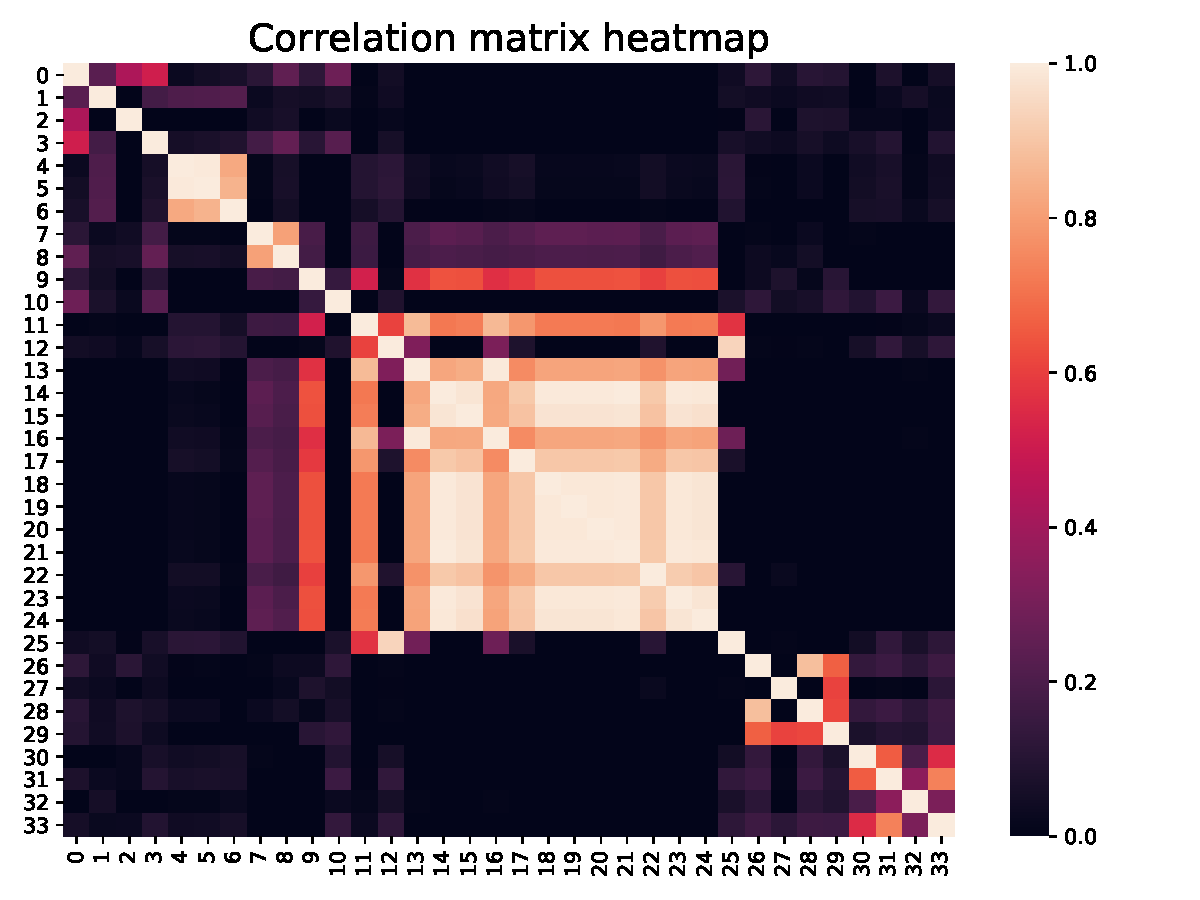
\includegraphics[width=1\linewidth]{images/corr_matrix}
	\caption{Matrice di correlazione delle feature del dataset. Legenda:
		0) Age,
		1) Number of sexual partners,
		2) First sexual intercourse,
		3) Num of pregnancies,
		4) Smokes,
		5) Smokes (years),
		6) Smokes (packs/year),
		7) Hormonal Contraceptives,
		8) Hormonal Contraceptives (years),
		9) IUD,
		10) IUD (years),
		11) STDs,
		12) STDs (number),
		13) STDs:condylomatosis,
		14) STDs:cervical condylomatosis,
		15) STDs:vaginal condylomatosis,
		16) STDs:vulvo-perineal condylomatosis,
		17) STDs:syphilis,
		18) STDs:pelvic inflammatory disease,
		19) STDs:genital herpes,
		20) STDs:molluscum contagiosum,
		21) STDs:AIDS,
		22) STDs:HIV,
		23) STDs:Hepatitis B,
		24) STDs:HPV,
		25) STDs: Number of diagnosis,
		26) Dx:Cancer,
		27) Dx:CIN,
		28) Dx:HPV,
		29) Dx,
		30) Hinselmann,
		31) Schiller,
		32) Citology,
		33) Biopsy.}
	\label{fig:corrmatrix}
\end{figure}

È stata quindi effettuata un'analisi più approfondita sui sample della classe positiva, ovvero che hanno ricevuto una diagnosi di cancro alla cervice uterina.
Grazie a informazioni apprese da siti informativi e di divulgazione \cite{veronesi}, è stato appreso come questa particolare forma di cancro sia spesso causata da una degenerazione del Papilloma virus, e che oltre al fumo, anche le malattie sessualmente trasmissibili costituiscono ulteriori fattori di rischio.
In Figura \ref{fig:dist} sono riportati i risultati delle analisi svolte sui sample con biopsia positiva.
Dalla Figura \ref{subfig:dist-age} si evince come il tumore abbia una forte incidenza nella fascia d'età $[18-33]$ anni; questo conferma le informazioni raccolte sui siti di divulgazione, dove si afferma che la fascia di età in cui questo tumore è maggiormente diffuso è tra i $20$ e i $30$ anni.
Analizzando la Figura \ref{subfig:dist-smoke} non troviamo invece conferma del fumo come un fattore di rischio rilevante: la maggioranza dei sample positivi non fuma, o fa un consumo minimo di sigarette durante l'anno.
Per quanto riguarda la relazione tra malattie sessualmente trasmissibili e lo sviluppo del cancro alla cervice, in Figura \ref{subfig:dist-stds} è possibile rilevare come oltre un terzo delle pazienti con biopsia positiva avessero effettivamente contratto nel passato almeno una malattia sessualmente trasmissibile.
Al contempo però, la Figura \ref{subfig:dist-hpv} sembra riportare un dato contrastante con le informazioni relative alla patologia: solo due pazienti malate hanno riportato di essere risultate positive al papilloma virus.\\
Al fine di interpretare correttamente questi dati, è necessario considerare due differenti condizioni: in primo luogo, il campione di pazienti presenti nel dataset che hanno sviluppato il cancro risulta essere molto esiguo (soli 54 individui).
Questo campione non permette quindi di poter trarre conclusioni o generalizzare circa la malattia, in quanto la ridotta dimensione potrebbe mostrare comportamenti o caratteristiche differenti dalla popolazione complessiva.
In secondo luogo, tutti i dati relativi all'anamnesi del paziente sono stati raccolti sotto forma di sondaggio; le risposte non possono essere quindi verificate e si affidano unicamente alla memoria/consapevolezza dei vari soggetti (\textit{i.e.}, un paziente potrebbe aver risposto di non avere malattie sessualmente trasmissibili a causa dell'assenza di una diagnosi di quest'ultima).
Gli studi effettuati devono quindi essere interpretati unicamente come un'analisi relativa alla distribuzione del campione analizzato e non possono essere generalizzati per trarre conclusioni circa il comportamento della malattia su una popolazione più ampia.
\begin{figure}[ht!]
	\centering
	\begin{tabular}{c}
		\subfloat[\label{subfig:dist-age} KDE (\textit{Kernel Density Estimation}) delle istanze appartenenti alla classe positiva al variare dell'età.]{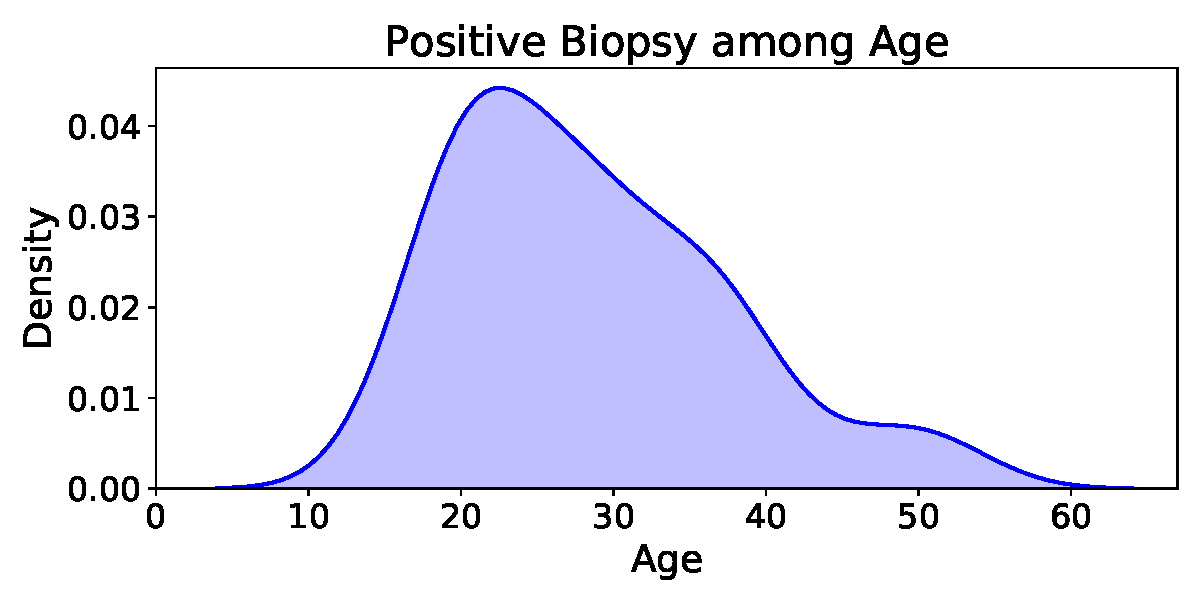
\includegraphics[width = 1\linewidth]{images/distribution_among_age}} \\
		\subfloat[\label{subfig:dist-smoke}KDE delle istanze appartenenti alla classe positiva al variare del numero di pacchetti di sigarette consumati all'anno.]{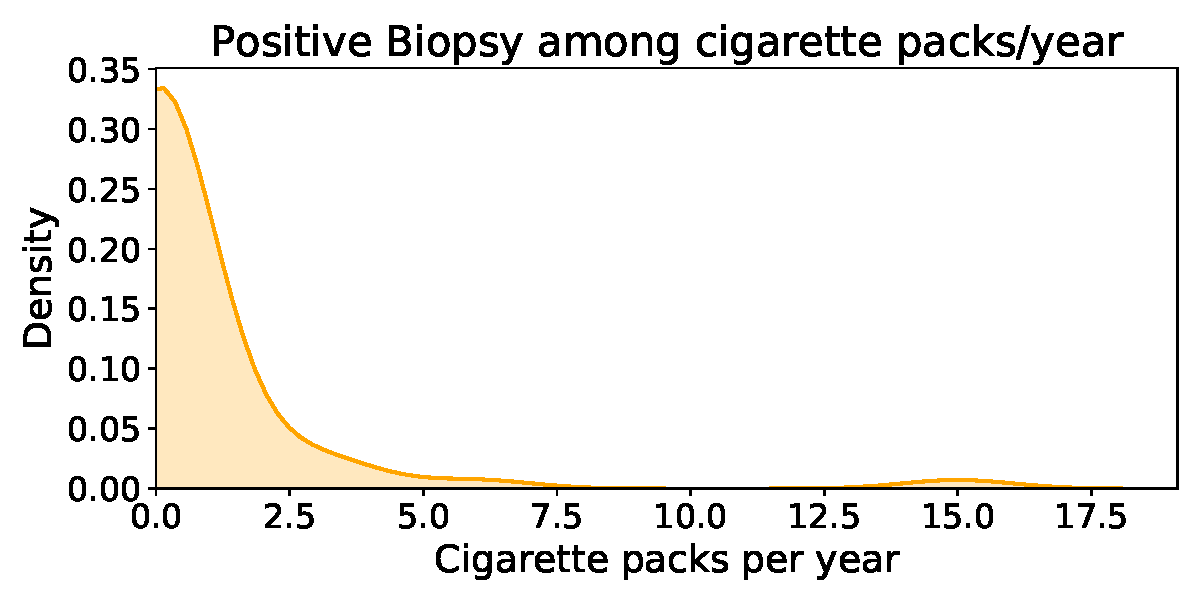
\includegraphics[width = 1\linewidth]{images/distribution_among_smoke}}
	\end{tabular}
	\begin{tabular}{cc}
		\subfloat[\label{subfig:dist-stds}Istogramma rappresentante la distribuzione dei soggetti affetti dalla patologia che hanno avuto almeno un malattia sessualmente trasmissibile.]{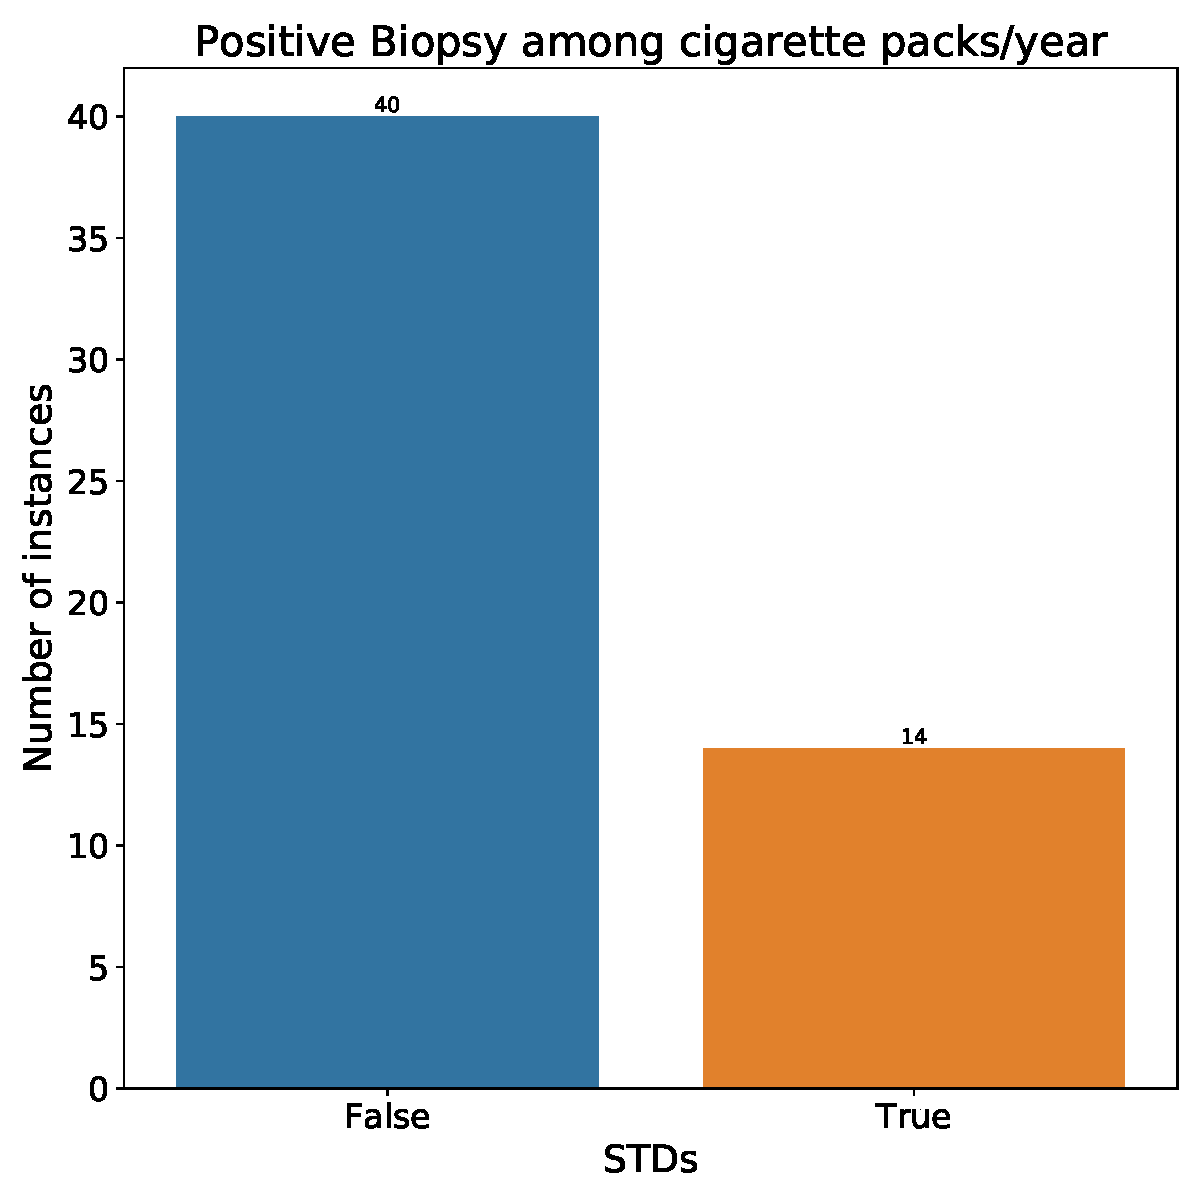
\includegraphics[width = .45\linewidth]{images/distribution_among_stds}} &
		\subfloat[\label{subfig:dist-hpv}Istogramma rappresentante la distribuzione dei soggetti affetti dalla patologia che hanno contratto il Papilloma Virus (HPV).]{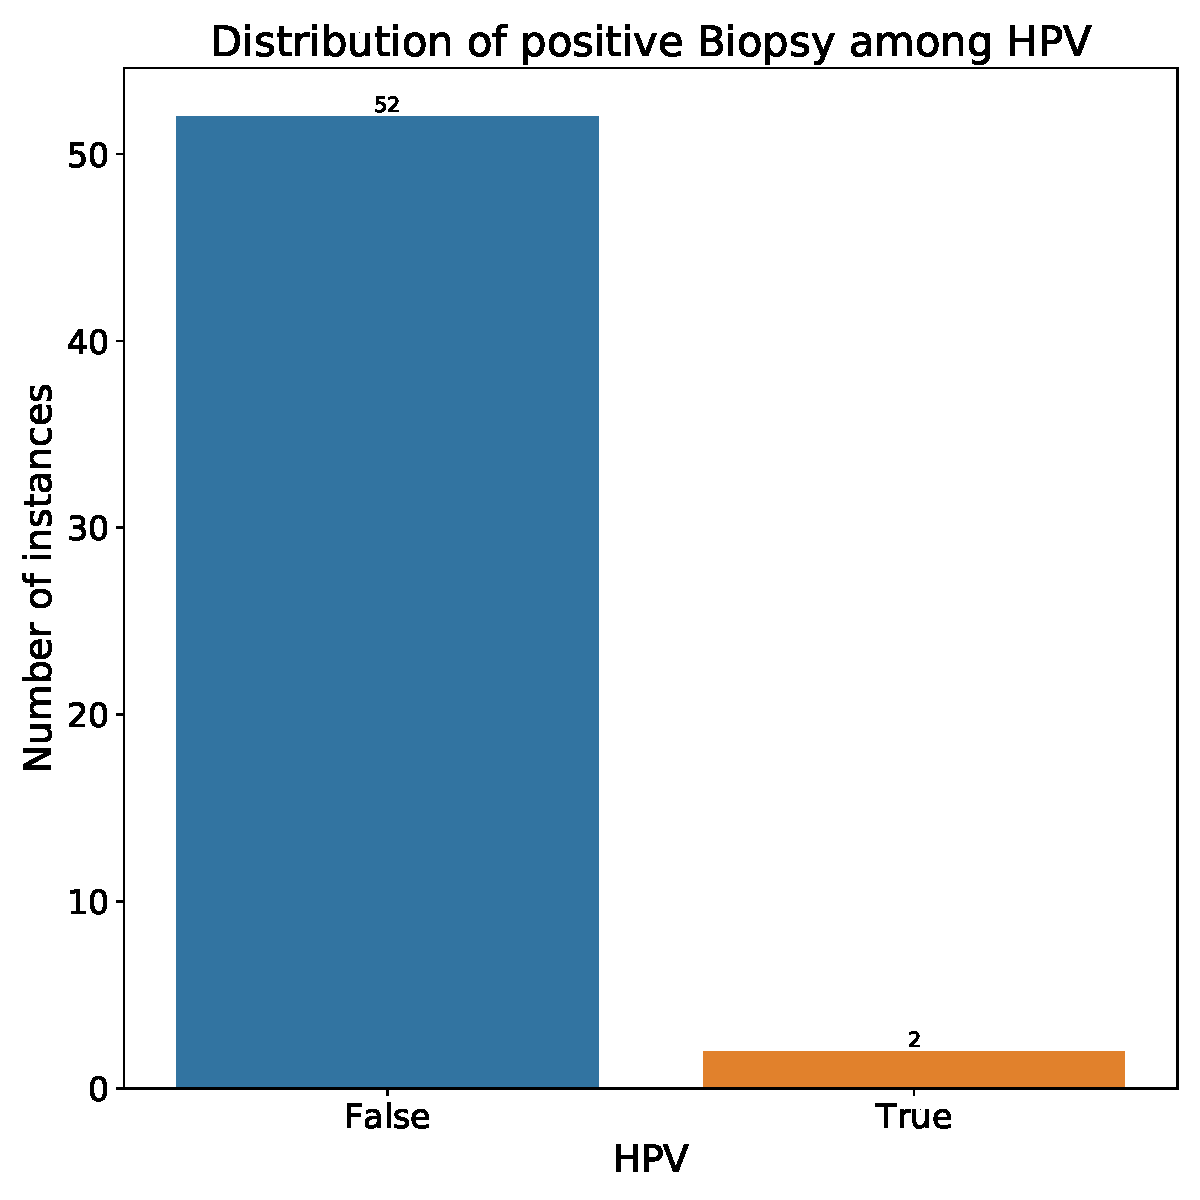
\includegraphics[width = .45\linewidth]{images/distribution_among_hpv}}
	\end{tabular}
	\caption{Distribuzione dei soggetti affetti dalla patologia rispetto a varie feature.}
	\label{fig:dist}
\end{figure}

\subsection{Data cleaning and preprocessing}
È stata dapprima indagata la presenza di valori mancanti nel dataset, rilevando come le due feature relative alla data della prima e ultima diagnosi di malattie sessualmente trasmissibili presentassero un numero elevatissimo di valori nulli.
Per questo motivo è stato deciso di rimuovere dal dataset questi dati, in quanto un tentativo di imputazione di questi valori si sarebbe dovuto basare su un numero di sample davvero esiguo. Non è invece stata rilevata la presenza di sample con un elevato numero di feature mancanti.
Il dataset è stato quindi diviso secondo l'etichetta ed è stata applicata una tecnica di imputazione per i \textit{missing value} dei due sottogruppi così generati: le feature intere sono state sostituite con la mediana dei valori, quelli booleani con la moda, mentre per i valori continui è stata utilizzato il valore medio arrotondato all'intero più vicino. Quest'ultima scelta è stata presa a seguito dell'analisi qualitativa dei dati, che ha mostrato come la stragrande maggioranza dei valori Double risultasse essere pari a 0 o ad un valore intero. Per questo motivo, al fine di non introdurre un'alterazione nel tipo dei dati presenti, è stata preferita una media arrotondata ad una più classica media semplice.
Dopo aver riunito il dataset, è stata effettuata una ricerca di outlier statistici.
Per fare ciò sono stati considerati unicamente le feature relative all'età delle pazienti e ai dati sull'attività sessuale. Non sono stati inclusi i dati circa le abitudini relative al consumo di sigarette o relativi agli anticoncezionali, in quanto si presenta un elevato numero di sample con valori associati a queste feature pari a $0$; il loro utilizzo avrebbe portato a considerare la maggioranza delle istanze con valori non nulli in questi campi degli outlier. Sono stati considerati outlier di una feature quei valori che superano di tre volte lo scarto interquantile. 
A seguito della rimozione dei sample considerati outlier per almeno una feature, il dataset presenta un totale di 776 sample per la classe negativa e 54 sample per la classe positiva, evidenziando come la maggioranza degli outlier sia stata individuata nella classe negativa.

\section{METODI}
\todo[inline]{controlla se ho messo numeri giusti, mi da errori quando carico il workflow di knime. please DP}
A seguito delle operazioni di \textit{preprocessing} del dataset, al fine di confrontare tra loro le varie tecniche di feature reduction, il \textit{workflow} si sviluppa in contemporanea su tre differenti livelli.
Ciascuno di essi gestisce privatamente una copia del dataset preprocessato.
Il primo livello fornisce in input agli algoritmi di apprendimento del modello il dataset senza che abbia subito alcuna operazione di feature reduction.
Il secondo fornisce come input all'algoritmo il risultato di un'operazione di feature extraction applicata al dataset mediante la tecnica della PCA (Principal Component Analysis). Questo approccio permette di trasformare un insieme di variabili correlate tra loro in un insieme ordinato di nuove feature non correlate tra loro; la trasformazione è definita in modo che la prima componente risulti essere quella con maggiore varianza, mentre tutte le successive mostrano il maggior valore di varianza possibile sotto il vincolo di ortogonalità con la precedente.
Al fine di stabilire la dimensionalità dello spazio di feature prodotto dalla PCA, è stato effettuato uno studio preliminare che consiste nella valutazione delle performance dei due algoritmi utilizzati (DT e RF) \todo{Se non citate prima mettere significato} al variare del numero di componenti nell'intervallo $[1, 33]$.
A seguito di questa analisi, la dimensione ottimale utilizzata è pari a 12, come suggerito dai risultati riportati in Figura \ref{fig:pca-perf}. Questo valore risulta essere un compromesso tra tra performance assolute e numero di feature prodotto; dal grafico è infatti possibile evincere come l'aumento della dimensionalità oltre le 12 feature garantisca un incremento delle prestazioni marginale e fortemente inconsistente.\\
Infine, il terzo livello del \textit{workflow} fornisce come input agli algoritmi di apprendimento automatico il dataset a seguito di un'operazione di feature selection mediante l'utilizzo di un filtro basato sulla correlazione; in particolare, gli attributi con una correlazione superiore a 0.85 sono stati rimossi. \todo[inline]{Per allungare il brodo potremmo fare uno studio al variare del threshold della fs come variano le performance? DP Più che altro è un incubo su knime visto come gestisce la cosa, ma si potrebbe fare, sembra interessante}
La scelta di tale filtro è stata dettata dal fatto che esso risulta appartenere alla classe dei filtri multivariati; ciò permette di individuare sia le feature irrilevanti sia quelle dipendenti tra loro, permettendo così di rimuovere la ridondanza dell'informazione. 
In aggiunta, i risultati evidenziati durante l'esplorazione del dataset (la presenza di feature altamente correlate tra loro) hanno suggerito la scelta di questa strategia, che risulta essere computazionalmente sostenibile dato il numero contenuto di record presenti nel dataset.

Per ogni livello del \textit{workflow} sono stati utilizzati due differenti algoritmi per apprendere i rispettivi modelli; in particolare sono stati impiegati un DT e una RF.
Per confrontare tali algoritmi \todo[inline]{il modello è quello che deriva dall'algoritmo, in una 5 fold ho di fatto 5 modelli, ma noi confrontiamo gli algo corretto? Dobbiamo essere molto attenti alla nomenclatura DP} è stato sfruttato un processo di 5-fold \textit{stratified cross-validation}.
La scelta di utilizzare una tecnica di \textit{cross-validation} stratificata (SCV) è stata dettata dalla natura estremamente sbilanciata del problema, che ha portato altresì alla scelta di utilizzare un numero di fold contenuto, paria a $5$, in modo da mantenere in ogni fold un numero ragionevole di esempi della classe minoritaria.
Data la scarsa rappresentazione della classe positiva presente nei vari train set, alla SCV è stata affiancata un'operazione di \textit{over-sampling} della classe minoritaria mediante la tecnica SMOTE (Synthetic Minority Over-sampling TEchnique). 
Questa tecnica permette di generare dei sample sintetici della classe minoritaria; gli attributi di ogni punto sintetico sono generati osservando i \textit{k nearest neighbors} di un sample e, dopo averne selezionato uno, il valore degli attributi è scelto casualmente nel range fissato dal valore dei due punti considerati.\todo{spiegare meglio, magari con una immagine}
L'operazione è stata effettuata esclusivamente sulla porzione di train di ogni iterazione della SCV, in modo da garantire che le performance misurate sul test set non fossero in alcuno modo influenzate.
L'utilizzo di una tecnica come SMOTE ha permesso di bilanciare le classi nei dati di training, permettendo così al modello di apprendere in modo più soddisfacente; è stato preferito l'\textit{over-sampling} all'\textit{under-sampling} in quanto quest'ultimo avrebbe ridotto drasticamente le dimensioni del train set, minando così le possibilità di apprendimento.
Si fa notare che il \textit{seed} per la generazione randomica dei fold è stato fissato a favore della ripetibilità dell'esperimento; tale \textit{seed} è inoltre condiviso tra tutti i generatori, in modo che vengano utilizzati i medesimi fold nei vari livelli del \textit{workflow}.
Al termine delle operazioni di \textit{cross-validation}, i modelli prodotti dagli algoritmi sono stati confrontati tra loro basandosi sulla misura f1-\textit{score} della classe minoritaria (\textit{i.e.}, presenza di cancro).
Si è scelto di utilizzare come metrica l'f1-\textit{score} perché in un problema del genere è stato ritenuto importante considerare sia la metrica di \textit{precision}, ovvero la percentuale di veri positivi individuati rispetto al totale di predizioni positive fatte, che la \textit{recall}, ovvero il numero di veri positivi individuati rispetto al numero totale che andava individuato. 
La motivazione alla base di questa decisione risulta essere chiara: si vorrebbero individuare correttamente il maggior numero possibile di soggetti affetti dalla patologia, mentre, al contempo, si vorrebbe evitare di diagnosticare erroneamente a molti pazienti di essere malati di cancro e costringerli così a dover affrontare ulteriori esami e operazioni invasive e costose; si è quindi optato per la medie armonica delle due metriche sopracitate (\textit{i.e.}, f1-\textit{score}), in modo da bilanciare i falsi positivi con i falsi negativi.
Un incontro con esperti del dominio medico potrebbe portare ad un cambio della misura di performance utilizzata, prediligendo una delle due componenti dell'f1-\textit{score} a discapito dell'altro; l'introduzione di una matrice dei costi che stimi il differente impatto economico e umano di falsi positivi e negativi potrebbe rivelarsi particolarmente utile in questo senso.\\
I confronti fra i vari modelli sono stati effettuati valutando la differenza tra la medie degli \textit{score} prodotti durante le varie iterazioni della \textit{cross-validation}; per stabilire se tale differenza fosse statisticamente significativa o meno sono stati utilizzati dei \textit{paired} t-test con un livello di confidenza pari a 0.95. Il test \textit{paired} è stato preferito alla versione \textit{unpaired} in quanto le performance dei vari modelli derivano i medesimi fold del processo di SCV.
Successivamente, sono stati confrontati fra loro i modelli ritenuti migliori per ogni livello (se sono risultati statisticamente differenti, altrimenti ne è stato selezionato uno a piacere), andando a verificare la presenza di un modello che risulti statisticamente migliore rispetto agli altri; anche questi test sono stati effettuati con un \textit{paired} t-test, con un valore di confidenza fissato a 0.95.

Infine, sono state valutate le performance di una RF in assenza di alcune feature derivanti da esami invasivi e costosi che, soprattutto in paesi di via di sviluppo, non risultano sempre disponibili o di facile accesso.
In particolare, dal dataset ottenuto a seguito della fase di preprocessing, sono state rimosse le seguenti feature: \textit{Hinselmann} (cioè la colposcopia), \textit{Schiller} (test eseguito durante la colposcopia) e \textit{Citology} (osservazione  al microscopio di cellule ottenute mediante il Pap test o altre tecniche).
Questo dataset è stato, quindi, utilizzato per l'esecuzione dell'algoritmo all'interno di una \textit{stratified 5-fold cross-validation} nelle stesse condizioni sperimentali presentate in precedenza.

\section{RISULTATI}
Per quanto concerne le analisi relative alle performance (in termini di f1-\textit{measure}, per i motivi precedentemente discussi) di DT e RF al variare del numero di feature estratte dal processo di PCA, i risultati (riportati in Figura \ref{fig:pca-perf}) mostrano come per un numero di componenti inferiore a $10$, le performance raggiunte dai modelli siano analoghe e pessime. Il trend si inverte con il raggiungimento della componente numero $12$, dove la tendenza varia completamente, portando le performance dei modelli ad assestarsi su valori decisamente migliori; dal grafico è possibile evincere come l'aumento della dimensionalità oltre le $12$ feature garantisca un incremento delle prestazioni marginale e fortemente inconsistente.
A seguito di questa analisi, la dimensione ottimale utilizzata è pari a $12$; questo valore risulta essere un compromesso tra performance assolute e numero di feature considerate.
In particolare si può notare come gli alberi di decisione inizino a mostrare un degradamento delle performance attorno alla componente $19$, portando ad una flessione delle f1-\textit{measure}, mentre le RF tendano a migliorare leggermente le loro predizioni, presentando però continue variazioni tra una dimensione e l'altra.\\
\begin{figure}
	\centering
	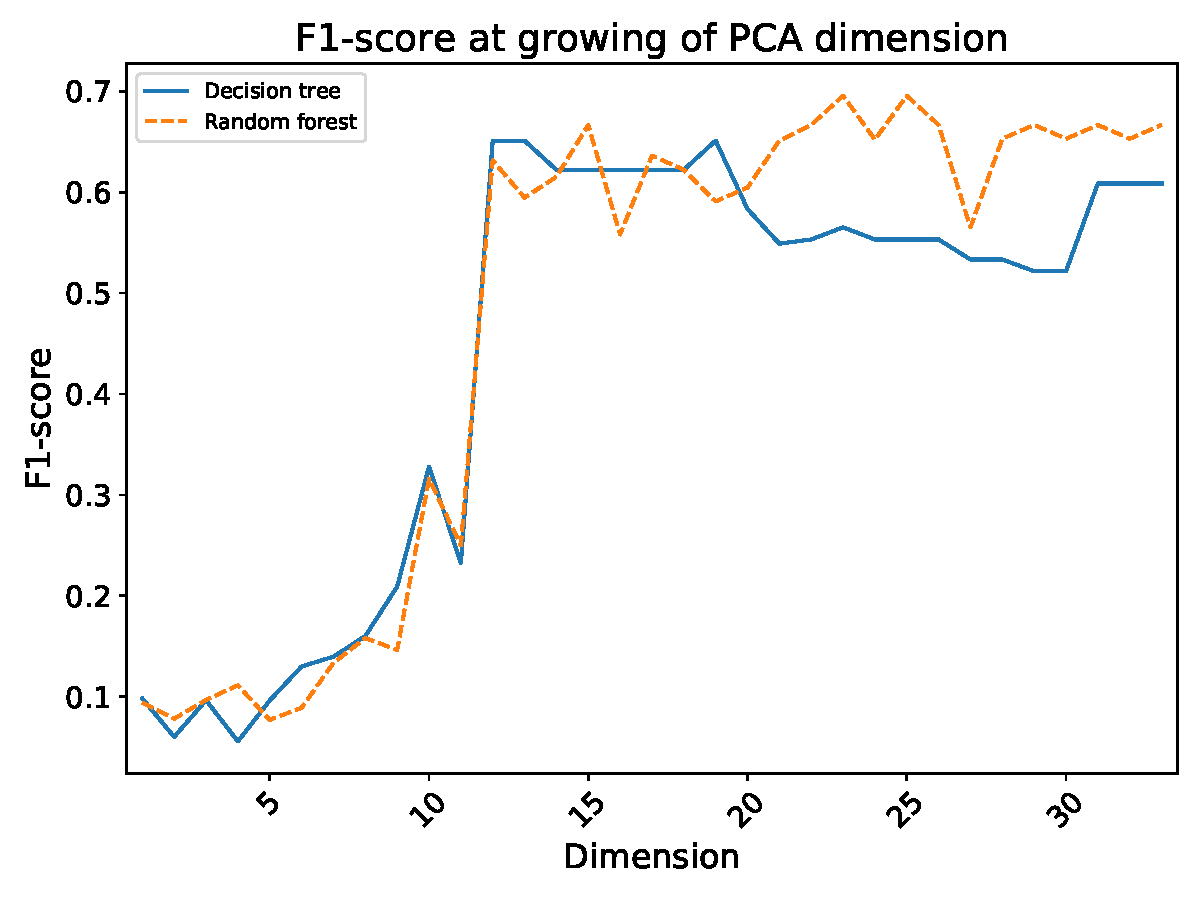
\includegraphics[width=1\linewidth]{images/pca-perf}
	\caption{Performance ottenute dai due modelli analizzati al crescere del numero di componenti della PCA utilizzate.}
	\label{fig:pca-perf}
\end{figure}
\todo[inline]{Sbaglio o non diciamo nei metodi che facciamo comunque una 5 fold stratiicata per il test sulla dimensione della PCA e non citiamo da nessuna parte che facciamo un test analogo con la soglia della feature selection su correlazione? DP}
La medesima analisi è stata effettuata sul grafico riportato in Figure \ref{fig:corr-perf} relativo ai risultati dei due modelli al variare del threshold di correlazione utilizzato nella feature selection. Sorprendentemente, la soglia corrispondente a valori ottimali è estremamente bassa, pari a $0.15$; questo valore porta alla rimozione di quasi tutte le feature del dataset, mantenendo solo 5 feature. Questo risultato porta a pensare che le feature del dataset siano fortemente correlate tra loro, costituendo in larga parte informazione ridondante. Anche in questo caso, come nel precedente, l'aggiunta di feature ulteriori sembra "distrarre" il classificatore, provocando un deterioramento delle performance significativo, salvo poi recuperare avvicinandosi alla situazione del dataset completo.
\begin{figure}
	\centering
	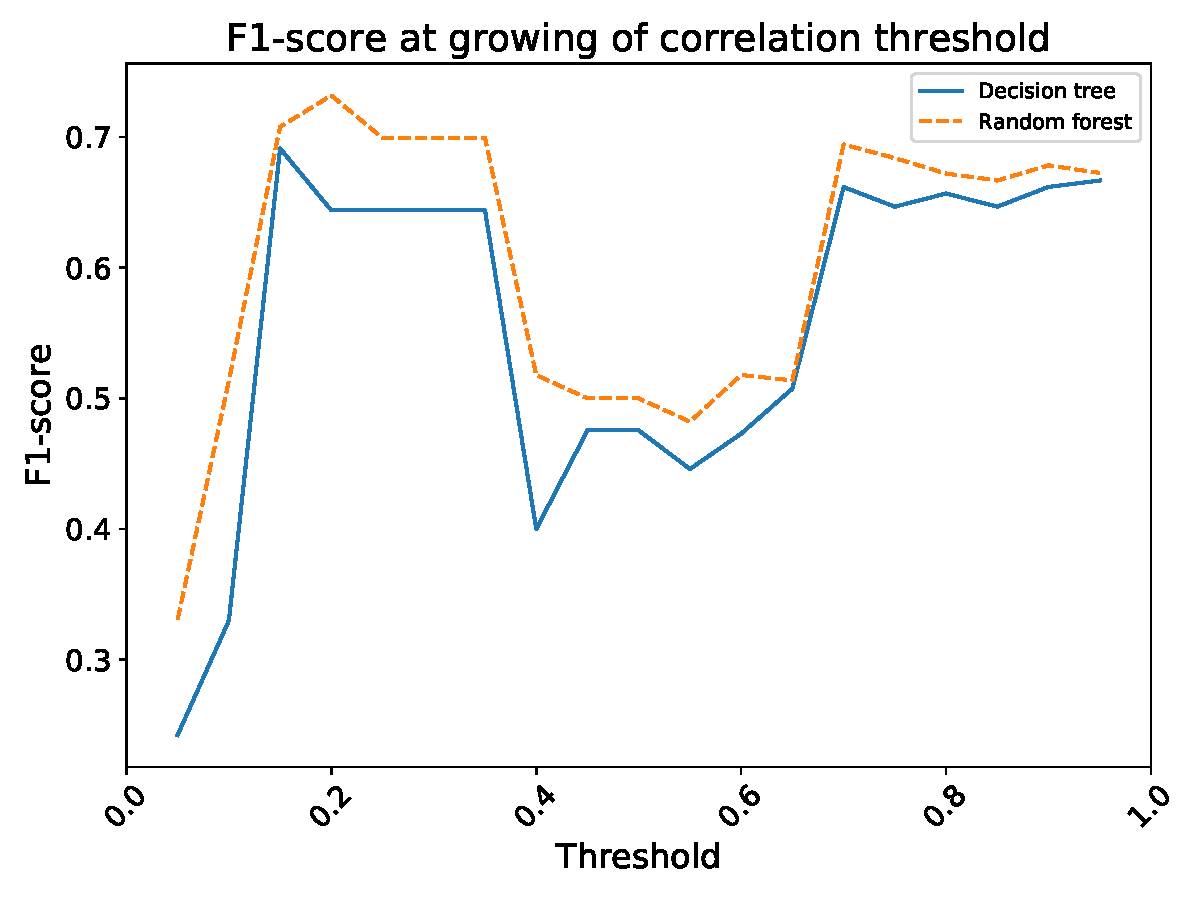
\includegraphics[width=1\linewidth]{images/corr-perf}
	\caption{Performance ottenute dai due modelli analizzati al crescere del valore di threshold del filtro di correlazione. Si noti che al crescere del valore di threshold, il numero di feature utilizzate cresce a sua volta.}
	\label{fig:corr-perf}
\end{figure}

Stabiliti quali fossero i parametri ottimali per le tecniche di \textit{feature reduction}, i vari algoritmi sono stati addestrati sui vari dataset prodotti. In particolare, per ogni input sono state testate sia alberi di decisione che random forest. Nel processo di train è stato deciso di utilizzare la tecnica di \textit{oversampling} in quanto i risultati di alcuni test preliminari effettuati hanno mostrato come l'utilizzo di tale approccio sia in grado di garantire in alcuni casi performance migliori rispetto alla versione non alterata del dataset. 
Nei casi restanti SMOTE è risultato semplicemente inefficace, senza indurre un peggioramento delle performance predittive.
\begin{table}
	\centering
	\caption{Performance medie del processo di 5-fold \textit{stratified cross-validation} sul dataset completo e dopo FR dei modelli analizzati.}
	\label{tab:f1score}
	\begin{tabular}{|c|c|c|}
		\toprule
		Modello & Tecnica da FR & f1-\textit{measure} media \\ 
		\midrule 
		Decision Tree & / & $0.647$ \\
		Random Forest & / & $0.715$ \\ 
		Decision Tree & Filtro correlazione & $0.607$ \\ 
		Random Forest & Filtro correlazione & $0.727$ \\ 
		Decision Tree & PCA & $0.691$ \\ 
		Random Forest & PCA & $0.74$ \\ 
		\bottomrule
	\end{tabular}
\end{table}
I risultati dei processi di SCV sono riportati in maniera analitica in Tabella \ref{tab:f1score} e nella Figura \ref{fig:fscore}, dalla quale è possibile notare come le performance medie dei modelli derivanti dalle random forest risultino essere migliori rispetto a quelli derivanti dagli alberi di decisione. Allo stesso modo è possibile notare come le performance medie migliori siano ottenete dal filtro delle feature basato sulla correlazione, mentre PCA e il dataset completo mostrano performance inferiori. 
\begin{figure}
	\centering
	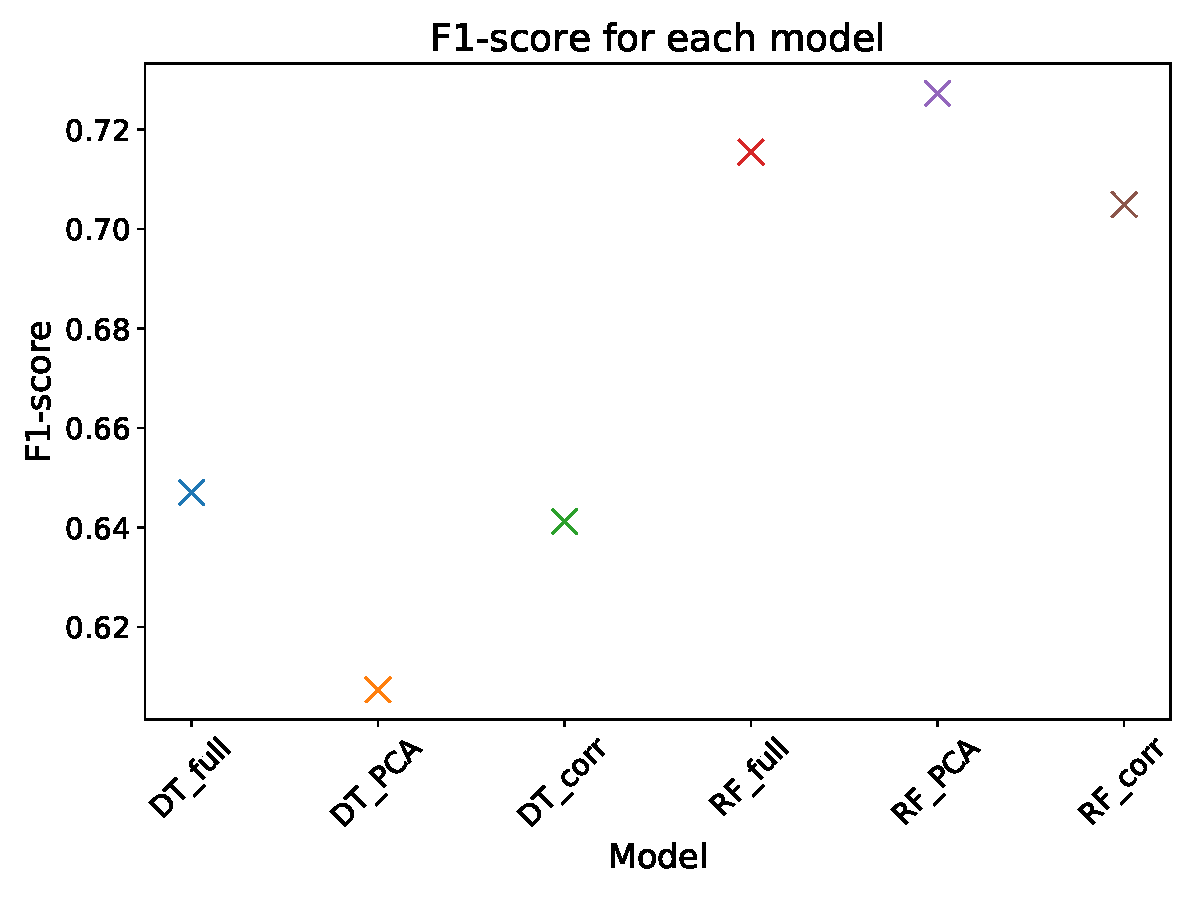
\includegraphics[width=1\linewidth]{images/fscore}
	\caption{Performance medie del processo di 5-fold \textit{stratified cross-validation} sul dataset completo e dopo FR dei modelli analizzati.}
	\label{fig:fscore}
\end{figure}
Al fine di stabilire se le differenze tra i vari modelli fossero statisticamente significative, è stato deciso di effettuare una serie di \textit{paired t-test} sulle performance dei vari modelli proposti nei vari fold della CV.
Analizzando in modo qualitativo i risultati associati ad ogni fold, è stata rilevata una forte eterogeneità nelle performance di ogni modello all'interno dei vari fold; un esempio di quanto affermato è riportato in Tabella \ref{tab:f1fold}, dove è possibile constatare come il range delle performance vari di oltre $20$ punti percentuali tra un fold e l'altro. Questo comportamento è probabilmente dovuto all'esiguo numero di sample disponibili, sia in fase di train che di test \todo[inline]{messa così è affermazione forte, io espanderei. DP}. Pur aumentando in maniera artificiale il numero di sample della classe minoritaria nel train set, i sample sintetici risulteranno molto simili a quelli già presenti nel train set e, se essi non sono una fedele rappresentazione della distribuzione reale dei dati a causa del numero limitato di sample a disposizione, l'algoritmo di apprendimento automatico non sarà in grado di generalizzare correttamente. 
\todo[inline]{Io aggiungere un altro esempio di performance, tanto spazio in più non lo occupiamo e facciamo vedere che non abbiamo preso il caso più sfigato DP}
\begin{table}
	\centering
	\caption{Performance ottenute dalla random forest con l'intero dataset in input nei vari fold della CV.}
	\label{tab:f1fold}
	\begin{tabular}{|c|c|}
		\hline 
		Fold & f1-\textit{measure} \\ 
		\hline 
		$1$ & $0.615$ \\ 
		\hline 
		$2$ & $0.846$ \\ 
		\hline 
		$3$ & $0.636$ \\ 
		\hline 
		$4$ & $0.692$ \\ 
		\hline 
		$5$ & $0.783$ \\ 
		\hline 
	\end{tabular} 
\end{table}
A conferma di quanto osservato, i test statistici non hanno evidenziato una differenza statisticamente rilevante tra le performance medie dei modelli DT e RF con input l'intero dataset e la riduzione tramite PCA. Al contrario, è emersa una differenza statisticamente rilevante tra le performance medie di alberi di decisione e random forset con input selezionato mediante correlazione. In questo caso, infatti, le RF mostrano performance statisticamente superiori agli alberi di decisione, come confermato dal test.
Lo studio è proseguito confrontando tra loro i modelli con input differenti; considerando i risultati dei test statistici appena presentati, è stato deciso di selezionare arbitrariamente le foreste per l'intero dataset e per la PCA (sarebbero stati allo stesso modo validi gli alberi di decisione, visto che non hanno mostrato performance medie statisticamente differenti), mentre per la tecnica di riduzione mediante correlazione è stata scelta la random forest in quanto mostrava performance migliori rispetto al corrispettivo albero di decisione. I risultati dei \textit{paired} t-test hanno mostrato nuovamente come non vi sia differenza statisticamente rilevante tra le performance medie dei modelli confrontati.
\todo{controllare che i t test dicano effettivamente questo MM}
\todo{Questi spazi continuano a farmi vomitare sempre più DP}
Un'ultima analisi realizzata in questo lavoro è stata come la rimozione delle feature relative agli esami clinici effettuati sulle pazienti potesse inficiare le performance predittive degli algoritmi di predizione considerati. Al dataset sono state rimosse le colonne \textit{Hinselmann, Schiller} e \textit{Citology}, ovvero i risultati dei 3 esami clinici effettuati sulle pazienti. Il processo di addestramento dei modelli è stato eseguito nelle medesime condizioni dei precedenti, ovvero utilizzando un processo di 5-fold \textit{stratified cross-validation} con \textit{oversampling} sul train set.
\todo[inline]{Tutto quello appena detto non l'abbiamo già detto nei metodi? perché ripeterlo? nel caso spostarlo sopra DP}
I risultati, riportati in Tabella \ref{tab:noexamsscore}, mostrano un drastico peggioramento delle performance predittive; ciò suggerisce che l'esecuzioni di questi esami (o di alcuni di essi) sia imprescindibile al fine di un corretto riconoscimento dei pazienti affetti dal cancro alla cervice da parte del modello. 
Risulta altresì improbabile la corretta classificazione di un paziente a partire unicamente dai relativi dati dell'anamnesi.
I risultati sono di particolare interesse se incrociati con quelli ottenuti nella fase di ricerca del threshold per il filtro basato sulla correlazione. In quello studio, il valore soglia proposto risultava molto basso, portando all'utilizzo di sole 5 feature che erano però in grado di garantire performance ottimali dei modelli. Tra di esse risulta presente la feature \textit{Schiller}, che viene invece rimosso nel test appena proposto, in cui le performance risultano pesantemente degradate. Possiamo quindi supporre che questa analisi porti con se una grande quantità di informazione; per questo motivo, nel caso in cui non fosse possibile eseguire tutti gli esami clinici proposti per motivi economici o tecnici, l'esecuzione del test di Schiller garantirebbe un sostanziale incremento delle performance del modello, portando così a predizioni più accurate.
Nonostante ciò, per quanto concerne i costi bisogna considerare che il test di Schiller avviene durante l'esecuzione della colposcopia, il cui esito è un'altra delle feature considerate.
\begin{table}
	\centering
	\caption{Performance medie del processo di \textit{stratified 5-fold cross-validation} dei modelli senza considerare le feature relative ad esami strumentali effettuati sulle pazienti.}
	\label{tab:noexamsscore}
	\begin{tabular}{|c|c|}
		\toprule
		Modello & f1-\textit{measure} media \\ 
		\midrule 
		Decision Tree & $0.201$ \\
		Random Forest & $0.165$ \\ 
		\bottomrule
	\end{tabular}
\end{table}

\addtolength{\textheight}{-7.5cm}

\section{CONCLUSIONI}


\begin{thebibliography}{99}

\bibitem{paper}
Kelwin Fernandes, Jaime S Cardoso, and Jessica Fernandes.
\textit{Transfer learning with partial observability applied to cervical cancer screening}.
Iberian conference on pattern recognition and image analysis, 243--250, 2017.

\bibitem{veronesi}
Fondazione Umberto Veronesi, Tumore della cervice uterina.
\url{https://www.fondazioneveronesi.it/magazine/tools-della-salute/glossario-delle-malattie/tumore-della-cervice-uterina-2}

\bibitem{ML}
UCI, Machine Learning Repository, Cervical cancer (Risk Factors) Data Set.
\url{https://archive.ics.uci.edu/ml/datasets/Cervical+cancer+\%28Risk+Factors\%29}


\end{thebibliography}

\end{document}
